\documentclass[14pt]{extbook}
\usepackage{multicol, enumerate, enumitem, hyperref, color, soul, setspace, parskip, fancyhdr} %General Packages
\usepackage{amssymb, amsthm, amsmath, latexsym, units, mathtools} %Math Packages
\everymath{\displaystyle} %All math in Display Style
% Packages with additional options
\usepackage[headsep=0.5cm,headheight=12pt, left=1 in,right= 1 in,top= 1 in,bottom= 1 in]{geometry}
\usepackage[usenames,dvipsnames]{xcolor}
\usepackage{dashrule}  % Package to use the command below to create lines between items
\newcommand{\litem}[1]{\item#1\hspace*{-1cm}\rule{\textwidth}{0.4pt}}
\pagestyle{fancy}
\lhead{Progress Quiz 7}
\chead{}
\rhead{Version A}
\lfoot{4173-5738}
\cfoot{}
\rfoot{Spring 2021}
\begin{document}

\begin{enumerate}
\litem{
Using the situation below, construct a linear model that describes the cost of the coffee beans $C(h)$ in terms of the weight of the high-quality coffee beans $h$.
\begin{center}
    \textit{ Veronica needs to prepare 210 of blended coffee beans selling for \$5.58 per pound. She has a high-quality bean that sells for \$6.69 a pound and a low-quality bean that sells for \$4.31 a pound. }
\end{center}
\begin{enumerate}[label=\Alph*.]
\item \( C(h) = -2.38 h + 1404.90 \)
\item \( C(h) = 2.38 h + 905.10 \)
\item \( C(h) = 5.50 h \)
\item \( C(h) = 6.69 h \)
\item \( \text{None of the above.} \)

\end{enumerate} }
\litem{
Determine the appropriate model for the graph of points below.
\begin{center}
    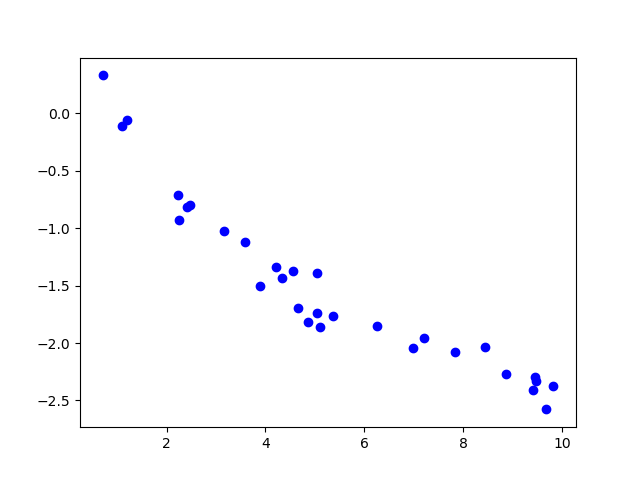
\includegraphics[width=0.5\textwidth]{../Figures/identifyModelGraph12CopyA.png}
\end{center}
\begin{enumerate}[label=\Alph*.]
\item \( \text{Logarithmic model} \)
\item \( \text{Non-linear Power model} \)
\item \( \text{Exponential model} \)
\item \( \text{Linear model} \)
\item \( \text{None of the above} \)

\end{enumerate} }
\litem{
Solve the modeling problem below, if possible.
\begin{center}
    \textit{ In CHM2045L, Brittany created a 30 liter 18 percent solution of chemical $\chi$ using two different solution percentages of chemical $\chi$. When she went to write her lab report, she realized she forgot to write the amount of each solution she used! If she remembers she used 10 percent and 36 percent solutions, what was the amount she used of the 10 percent solution? }
\end{center}
\begin{enumerate}[label=\Alph*.]
\item \( 9.23 \)
\item \( 15.00 \)
\item \( 10.90 \)
\item \( 20.77 \)
\item \( \text{There is not enough information to solve the problem.} \)

\end{enumerate} }
\litem{
Solve the modeling problem below, if possible.
\begin{center}
    \textit{ A new virus is spreading throughout the world. There were initially 4 many cases reported, but the number of confirmed cases has doubled every 4 days. How long will it be until there are at least 10000 confirmed cases? }
\end{center}
\begin{enumerate}[label=\Alph*.]
\item \( \text{About } 32 \text{ days} \)
\item \( \text{About } 18 \text{ days} \)
\item \( \text{About } 46 \text{ days} \)
\item \( \text{About } 16 \text{ days} \)
\item \( \text{There is not enough information to solve the problem.} \)

\end{enumerate} }
\litem{
For the scenario below, use the model for the volume of a cylinder as $V = \pi r^2 h$.
\begin{center}
    \textit{ Pringles wants to add 42 \text{percent} more chips to their cylinder cans and minimize the design change of their cans. They've decided that the best way to minimize the design change is to increase the radius and height by the same percentage. What should this increase be? }
\end{center}
\begin{enumerate}[label=\Alph*.]
\item \( \text{About } 3 \text{ percent} \)
\item \( \text{About } 19 \text{ percent} \)
\item \( \text{About } 21 \text{ percent} \)
\item \( \text{About } 12 \text{ percent} \)
\item \( \text{None of the above} \)

\end{enumerate} }
\litem{
Solve the modeling problem below, if possible.
\begin{center}
    \textit{ In CHM2045L, Brittany created a 29 liter 32 percent solution of chemical $\chi$ using two different solution percentages of chemical $\chi$. When she went to write her lab report, she realized she forgot to write the amount of each solution she used! If she remembers she used 13 percent and 37 percent solutions, what was the amount she used of the 13 percent solution? }
\end{center}
\begin{enumerate}[label=\Alph*.]
\item \( 14.50 \)
\item \( 22.96 \)
\item \( 6.04 \)
\item \( 8.00 \)
\item \( \text{There is not enough information to solve the problem.} \)

\end{enumerate} }
\litem{
Solve the modeling problem below, if possible.
\begin{center}
    \textit{ A new virus is spreading throughout the world. There were initially 6 many cases reported, but the number of confirmed cases has doubled every 3 days. How long will it be until there are at least 10000 confirmed cases? }
\end{center}
\begin{enumerate}[label=\Alph*.]
\item \( \text{About } 10 \text{ days} \)
\item \( \text{About } 23 \text{ days} \)
\item \( \text{About } 12 \text{ days} \)
\item \( \text{About } 33 \text{ days} \)
\item \( \text{There is not enough information to solve the problem.} \)

\end{enumerate} }
\litem{
For the scenario below, use the model for the volume of a cylinder as $V = \pi r^2 h$.
\begin{center}
    \textit{ Pringles wants to add 27 \text{percent} more chips to their cylinder cans and minimize the design change of their cans. They've decided that the best way to minimize the design change is to increase the radius and height by the same percentage. What should this increase be? }
\end{center}
\begin{enumerate}[label=\Alph*.]
\item \( \text{About } 14 \text{ percent} \)
\item \( \text{About } 8 \text{ percent} \)
\item \( \text{About } 13 \text{ percent} \)
\item \( \text{About } 3 \text{ percent} \)
\item \( \text{None of the above} \)

\end{enumerate} }
\litem{
Using the situation below, construct a linear model that describes the cost of the coffee beans $C(h)$ in terms of the weight of the low-quality coffee beans $h$.
\begin{center}
    \textit{ Veronica needs to prepare 230 of blended coffee beans selling for \$4.70 per pound. She has a high-quality bean that sells for \$6.55 a pound and a low-quality bean that sells for \$3.99 a pound. }
\end{center}
\begin{enumerate}[label=\Alph*.]
\item \( C(h) = 5.27 h \)
\item \( C(h) = -2.56 h + 1506.50 \)
\item \( C(h) = 2.56 h + 917.70 \)
\item \( C(h) = 3.99 h \)
\item \( \text{None of the above.} \)

\end{enumerate} }
\litem{
Determine the appropriate model for the graph of points below.
\begin{center}
    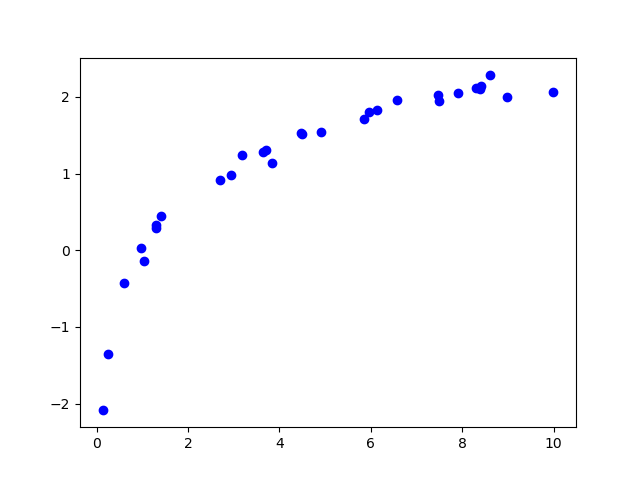
\includegraphics[width=0.5\textwidth]{../Figures/identifyModelGraph12A.png}
\end{center}
\begin{enumerate}[label=\Alph*.]
\item \( \text{Linear model} \)
\item \( \text{Non-linear Power model} \)
\item \( \text{Exponential model} \)
\item \( \text{Logarithmic model} \)
\item \( \text{None of the above} \)

\end{enumerate} }
\end{enumerate}

\end{document}